\subsection{Einführung}
\label{subsec:delaunay-introduction}

Wie in~\cite{atsuyuki2000spatialtessellations} angegeben, kann aus einem gegeben, $m$-dimensionalen Voronoi-Diagramm ein weiteres, zum Voronoi-Diagramm duales Diagramm abgeleitet werden. Es handelt sich dabei um die Delaunay-Tesselation bzw. -Triangulation. Dabei werden die Punkte, deren Regionen eine $(m-1)$-dimensionale Oberfläche teilen, verbunden.

Die Delaunay-Tesselation kann allerdings auch direkt aus der Punktemenge erstellt werden, indem jeweils der Umkreis von $(m+1)$ Punkten betrachtet wird. Befindet sich keiner der Puntke aus der Menge in der Fläche des Kreises, wird ein Simplex aus den $(m+1)$ Punkten gebildet. Befindet sich ein Punkt in der Fläche, wird nichts unternommen. Dies geschieht so lange, bis alle möglichen Flächen über $(m+1)$ Punkte gebildet wurden.

\begin{figure}[h]
\centering
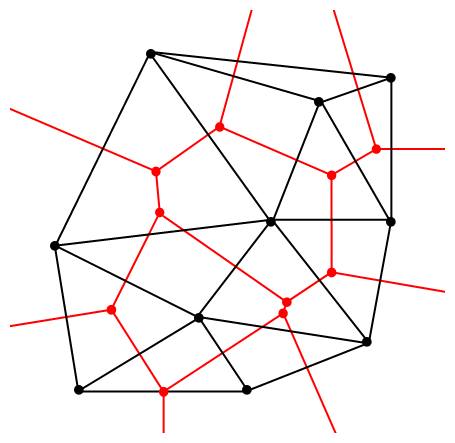
\includegraphics[width=130px]{images/voronoi_delaunay_example_01.png}
\caption{Beispiel einer Delaunay-Triangulation (schwarz) anhand eines Voronoidiagramms (rot)}
\label{fig:delaunayVoronoiExample}
\end{figure}


In der Computergrafik werden in der Regel Polygone verwendet um 2D- oder auch 3D-Modelle darzustellen, sprich, zu rendern. Um diese Modelle möglichst schnell und effizient darzustellen wird bei den Grafikkarten stark auf Optimierung gesetzt. So wird eine Fläche, welche aus Dreiecken besteht, sehr effizient dargestellt. Dies, da ein Dreieck aus drei Punkten besteht und alle diese Punkte auf der selben Ebene liegen, was den Vorgang der Rasterisierung (vereinfacht, die Darstellung einer n-dimensionalen Szene auf einer zweidimensionalen Fläche) deutlich vereinfacht.

Die Delaunay-Triangulation ermöglicht es auf eine effiziente Weise beliebige Flächen zu triangulieren. Wie bereits in~\ref{sec:introduction} erwähnt, kann dies beispielsweise dazu genutzt werden um eine Oberfläche in einem Geoinformationssystem oder ein Polygonnetz zur Darstellung eines dreidimensionalen Modells in einer in Echtzeit auf digitaler Hardware erzeugten multimedialen Präsentation zu erzeugen.

\begin{figure}[h]
\centering
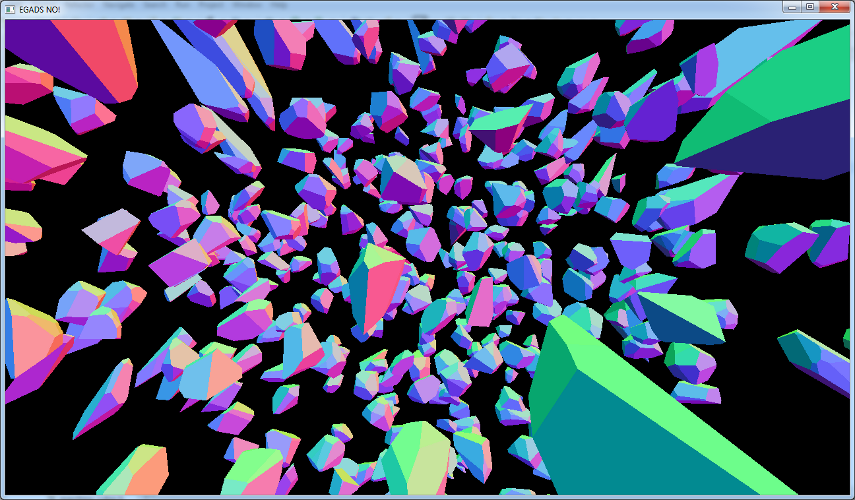
\includegraphics[width=200px]{images/voronoi_delaunay_example_02.png}
\caption[width=100px]{Beispiel von Polygon-Modellen, welche mit Delaunay-Triangulation erzeugt wurden}
\label{fig:delaunayVoronoiExample2}
\end{figure}
